\chapter*{Prefacio}
Estas notas son una transcripción (libremente adaptada) de las clases de la asignatura ``\ti{Investigación Operativa}'', impartidas por María Inés Sobrón Fernández en el curso 2016--2017 a los cursos de cuarto y tercero de los dobles grados de  Matemáticas -- Física e Ingeniería Informática -- Matemáticas (respectivamente) en la facultad de Ciencias Matemáticas de la Universidad Complutense de Madrid (UCM).

Cualquier aportación o sugerencia de mejora es siempre bienvenida.
\subsection*{Requisitos previos}
Para comprender estas notas en su totalidad es necesario tener soltura a la hora de trabajar con bases de espacios vectoriales de dimensión finita y comprender bien las aplicaciones lineales. También es bastante recomendable recordar algunos aspectos del cálculo diferencial en varias variables, no obstante, el texto es bastante autocontenido en ese aspecto.
%\subsection*{Nota del autor}
\subsection*{Agradecimientos}
La existencia de estas notas es debida a la amabilidad de Clara Rodríguez Núñez, quien me cedió sus apuntes tomados durante el curso, en los cuales se basa el núcleo de este texto.
\subsection*{Licencia}
Esta obra está sujeta a la licencia Reconocimiento-NoComercial-CompartirIgual 4.0 Internacional de Creative Commons. Para ver una copia de esta licencia, visite \url{http://creativecommons.org/licenses/by-nc-sa/4.0/}.
\begin{figure}[h]
	\centering
	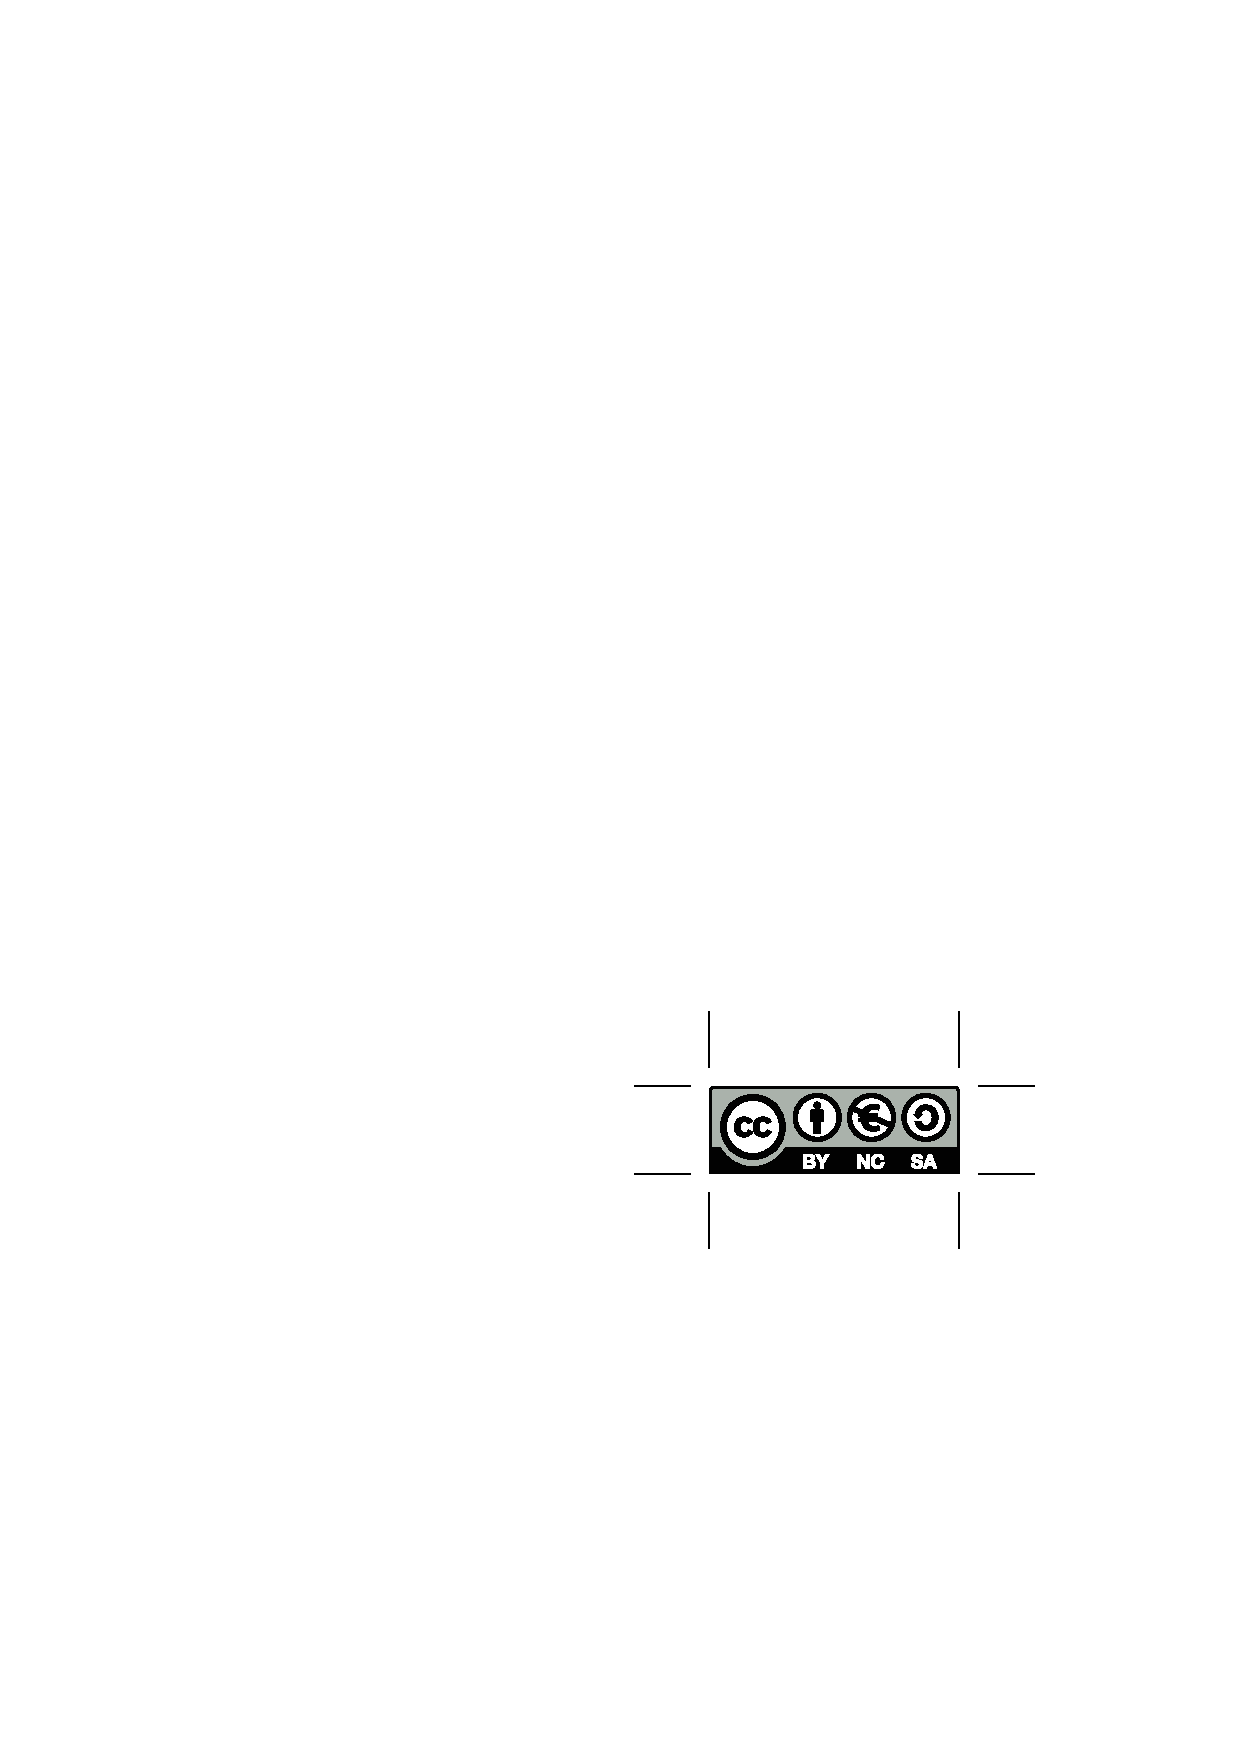
\includegraphics[scale=1]{img/licencia}
\end{figure}

El código fuente de este documento es de libre acceso y se encuentra alojado en \url{https://github.com/alvarogatenorio/Investigacion-Operativa} paro uso y disfrute de todo el que quiera, siempre que se respeten los términos de la licencia.